\tikzsetnextfilename{barr_blocks_annotated}%
\begin{tikzpicture}
    \node[above right, inner sep=0] (image) at (0,0) {
        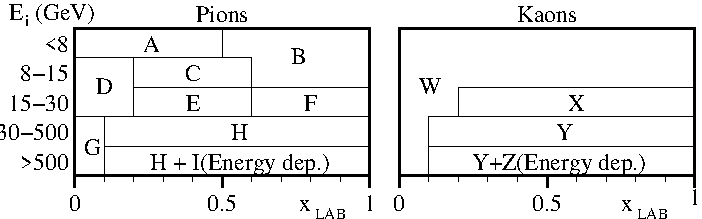
\includegraphics[width=0.8\linewidth]{figures/measurement/systematics/flux/barr_blocks.pdf}
    };
    % Create scope where axes are matching the Pion grid
    \begin{scope}[
        x={($0.42*(image.south east)$)},
        y={($0.67*(image.north west)$)},
        shift={($0.107*(image.south east) + 0.2*(image.north west)$)}
    ]
        % Grid
        %\draw[darkgray,step=0.2] (0,0) grid (1,1);
        \draw[thick, orange, fill=orange, fill opacity=0.8] (0, 0.4) rectangle (1, 1);
        \node[anchor=south, fill=white, draw=black] at (0.5, 0.55) {merged A-F};
    \end{scope}
\end{tikzpicture}